\documentclass[conference]{IEEEconf}
\IEEEoverridecommandlockouts

\usepackage{cite}
\usepackage{amsmath,amssymb,amsfonts}
\usepackage{amsthm}
\usepackage{algorithm}
\usepackage{algorithmic}
\usepackage{graphicx}
\usepackage{booktabs}
\usepackage[hidelinks]{hyperref}
\usepackage{textcomp}
\usepackage{xcolor}
\usepackage{float}     % enables [H]
\usepackage{placeins}  % enables \FloatBarrier
\def\BibTeX{{\rm B\kern-.05em{\sc i\kern-.025em b}\kern-.08em
    T\kern-.1667em\lower.7ex\hbox{E}\kern-.125emX}}

\DeclareMathOperator{\degr}{deg}     % degree operator: \degr(i)
\newcommand{\Ni}{\mathcal{N}}        % neighbor set: \Ni(i)
\newcommand{\CN}[2]{\Ni(#1)\cap\Ni(#2)} % common neighbors: \CN{i}{j}
\newcommand{\Nii}[1]{\Ni^{(2)}(#1)}  % 2-hop neighbors

\renewcommand{\algorithmicrequire}{\textbf{Input:}}
\renewcommand{\algorithmicensure}{\textbf{Output:}}

\newcommand{\xyu}[1]{\textcolor{magenta}{#1}}

\theoremstyle{plain}
\newtheorem{assumption}{Assumption}
\newtheorem{theorem}{Theorem} 
\newtheorem{lemma}{Lemma}
\newtheorem{definition}{Definition}
\newtheorem{example}{Example}
\newtheorem{remark}{Remark}

\title{\LARGE \bf
Distributed Control and Communication Framework for Connectivity Preservation in Flow-Driven Robot Fleets}
\author{Prajjwal Dutta, Geoff Hollinger, and Xi Yu\\
 \thanks{This work was supported by the NSF Awards 2322055 and 2529791.}
 \thanks{P. Dutta and X. Yu is with the School of Manufacturing Systems and Networks at Arizona State University (e-mail: \{pdutta9, xyu\}@asu.edu).
 G. Holinger is with the Department of Mechanical, Industrial, and Manufacturing Engineering at Oregon State University (e-mail: Geoff.Hollinger@oregonstate.edu).
}
 }

\begin{document}

\maketitle

\begin{abstract}
We consider deployment of underwater robot fleets in flow-dominated environments where communication is short-range and unreliable, localization may be denied, and actuation energy is limited. The key systems challenge is to maintain end-to-end connectivity under flow-driven dispersion while executing a mission objective, under realistic communication constraints.

We propose a two-layer architecture. First, a distributed topology-maintenance layer sparsifies the time-varying communication graph to a connected, spanning-tree-like subgraph using only local neighbor exchanges. In contrast to communication-heavy graph methods, the topology layer relies on constant-size messages and local parent selection to prune redundant edges; we explicitly account for bytes per message, messages per update, and delivered bandwidth, and evaluate robustness under packet drops, random delays, asynchronous broadcasts, and neighbor churn. Second, each robot solves a standard Controlled Lyapunov Functions (CLFs) and Controlled Barrier Functions (CBFs) with quadratic program (QP) that minimally modifies a nominal goal-seeking controller to satisfy collision-avoidance and range-maintenance constraints on the maintained edges.

We validate the complete pipeline in 3D HoloOcean simulations with multiple BlueROV2 vehicles under an advection--diffusion motion model, demonstrating goal-directed navigation while preserving end-to-end connectivity with measured communication budgets under impaired channels.
\end{abstract}

\section{Introduction}\label{sec:intro}

We are interested in deploying a fleet of underwater robots into large-scale, challenging environments such as the deep ocean and under-ice cavities, where localization is denied, communication bandwidth is limited, and the environment is dominated by dynamic flows and eddies \cite{muto2024}. 
These robots must traverse long distances on limited energy budgets, discover emerging regions of interest, sample the environment, and relay data, all while relying on intermittent and bandwidth-limited communication \cite{schiel2024chirps, schiel2024role}.

The central challenge is to design strategies that enable the fleet to (i) efficiently cover a large spatial domain to discover emerging targets while maintaining network connectivity, and (ii) realize a globally connected configuration using only localized information and limited communication.

Our proposed approach is to deploy the robots together and then allow them to drift with the prevailing flow . Control effort is only applied when it is necessary. This includes situations when the robots risk drifting outside a prescribed region or when they risk losing connectivity. In this way the formation disperses while staying connected, and the group can also reconfigure when a new target location is discovered or generated \cite{butler2025}. This strategy is bold, but it is supported by recent progress. Previous work has shown that surface vehicles can drift with the flow while using minimal control to remain in gyre like structures \cite{wei2019}, or track the periodicity of revisits via intermittent control triggered by prescribed conditions \cite{knizhnik2022}. In addition, broadly adopted models describe the uncontrolled motion of objects in water as drift combined with Brownian type diffusion \cite{taylor1922, okubo1971, majda1999}, which align with observation on underwater robots \cite{berlinger2021, quattrini2023}. This indicates that our fleet will approximately follow the main direction of the flow while also dispersing stochastically.

Although dispersion promotes coverage of large task spaces, two challenges remain open. The first is how to maintain connectivity. The second is how to enable reconfiguration around targets while working with unreliable communication that cannot support centralized control. Prior work on connectivity maintenance and target surrounding has emphasized the importance of graph theoretic methods \cite{olfati2007,dimartino2006}. Control barrier functions (CBFs) have received attention for their energy efficiency in this setting. For example, CBFs have been applied to the Fiedler value of the network graph in order to maintain connectivity \cite{capelli2020}. This approach is effective but it requires centralized and computationally expensive eigenvalue calculations. Other work has applied distributed CBF formulations that keep robots pairwise within communication range \cite{sabattini2013,capelli2021}. More recently, a hybrid framework was introduced that combines distributed CBFs with a graph theoretic tool, where each robot interacts only with a limited set of neighbors defined by a minimum spanning tree (MST) \cite{yang2023}. This solution is promising since each robot only applies CBF to itself and to selected neighbors, but it still requires generating a minimum spanning tree that depends on global information.

In our case a feasible framework must combine two ingredients. The first is a distributed neighbor selection strategy so that each robot chooses a limited set of neighbors to remain within communication range. The second is a local control law applied only to these neighbors. Together these two features must guarantee global connectivity. Work on spanning trees has shown that distributed verification methods exist, but the actual construction of a minimum spanning tree is classically centralized \cite{boruvka1926, kruskal1956, prim1957}. Progress in fully distributed protocol for exact MST construction \cite{gallager1983, awerbuch1987} remain communication-intensive. As a result, several approximate or near-optimal distributed methods have been proposed, but they do not achieve exact solutions \cite{khan2008}.

We take advantage of two features of our setting. First, the robots are deployed together so the initial configuration is connected. Second, the purpose of sparsifying the communication graph is to reduce unnecessary long-range maintenance. A robot should drop links to distant neighbors whenever connectivity can be preserved through closer neighbors at lower control and communication cost. Recent progress has also shown that robots can identify connectivity-relevant structure using distributed procedures with limited information exchange \cite{venkateswaran2024}. Motivated by these observations, we design a distributed topology-maintenance layer that constructs a sparse spanning-tree coordination structure and prunes redundant edges using only local neighbor broadcasts, with explicit accounting of message size and update frequency.

Upon this maintained structure, we apply a standard control Lyapunov function--control barrier function (CLF--CBF) controller. The CLF term captures nominal goal-seeking behavior, while CBF constraints enforce (i) collision avoidance and (ii) communication-range maintenance \emph{only} on the maintained links. When a target is detected, the detecting robot moves toward the target and the remaining robots reconfigure to preserve a connected support network during motion under flow-driven dispersion.

\textbf{Systems contributions} (i) A communication-feasible distributed pruning protocol that constructs a connected spanning-tree topology with constant-size messages per broadcast and local keep/prune decisions, together with measured communication budgets. (ii) A closed-loop integration of topology maintenance with CLF--CBF control for goal-reaching under link-maintenance constraints on the maintained tree edges. (iii) A 3D simulation evaluation in HoloOcean with BlueROV2 vehicles under an advection--diffusion motion model, including packet drops, random delays, asynchronous updates, and neighbor churn.

This paper is organized as follows. Sec.~\ref{sec:prob} introduces the problem and modeling assumptions. Sec.~III presents the distributed topology-maintenance protocol and the CLF--CBF control layer. Sec.~IV describes the communication model and experimental setup (including drops, delays, and asynchronous updates). Sec.~V reports simulation results in both synthetic graphs and 3D HoloOcean, and discusses communication cost and robustness. Sec.~VI concludes and outlines limitations.

\section{Background and Problem Formulation}\label{sec:prob}

We now formalize the problem. This section introduces the robot dynamics model, states the assumptions, defines the graph-theoretic notation, and presents the formal problem statement.
\subsection{Advection-diffusion model \cite{taylor1922, okubo1971, majda1999}}

We model a fleet of $N$ robots operating in $\mathbb{R}^n$ (with $n=2$, used for visualization in our simulations) released together in the water, their collective motion can be decomposed into a drift component induced by an ambient flow field and a stochastic dispersion component due to unexpected turbulence and small perturbations. Let $x_i(t) \in \mathbb{R}^n$ denote the position of the $i$-th robot at time $t$, where $i\in \{1,2,...,N\}$, and let  
\[
\bar{x}(t) = \frac{1}{N} \sum_{i=1}^N x_i(t)
\]  
be the center of mass of the group. 

The evolution of the center of mass is governed primarily by the advective flow field, i.e.,  
\[
\dot{\bar{x}}(t) \approx f_{\text{flow}}(\bar{x}(t),t),
\]  
where $f_{\text{flow}}$ is the background velocity field. Each individual object then deviates from $\bar{x}(t)$ due to unresolved small-scale turbulence and fluctuations, which can be modeled as Brownian motion:  
\begin{equation}
\begin{gathered}
    dx_i(t) = (f_{\text{flow}}(x_i(t), t) + v_i(t)) dt + \sigma_{\text{diff}} dW_i(t) \\
    \dot{v}_i(t) = u_i(t) - \gamma v_i(t)
\end{gathered}
\label{eq:advec_diff}
\end{equation}
\noindent where $v_i(t) \in \mathbb{R}^n$ is the velocity of each individual robot, $u_i(t) \in \mathbb{R}^n$ is the thrust, $\gamma > 0$ is a velocity damping factor, and $W_i(t)$ is a Wiener process capturing diffusion (with intensity $\sigma_{\text{diff}}$).

Thus the group drifts together with the flow through the motion of $\bar{x}(t)$, while individuals spread stochastically around the drifting center due to the independent diffusion terms.

\noindent\textbf{Discrete-time simulation (Euler--Maruyama).}
In simulation we integrate~\eqref{eq:advec_diff} using Euler--Maruyama with step $\Delta t$:
\begin{equation}
\begin{aligned}
x_i^{k+1} &= x_i^k + \big(f_{\mathrm{flow}}(x_i^k,t_k)+v_i^k\big)\Delta t
           + \sigma_{\mathrm{diff}}\sqrt{\Delta t}\,\xi_i^k,\\
\xi_i^k &\sim \mathcal{N}(0,I).
\end{aligned}
\label{eq:em}
\end{equation}
together with the velocity update $v_i^{k+1}=v_i^k+\big(u_i^k-\gamma v_i^k\big)\Delta t$.
This makes the diffusion term an explicit part of the state evolution used in our experimental evaluation.

As an example, the flow field is a base current plus a spatially varying swirl:
\begin{equation*}
f_{\text{flow}}(x,t) = v_{\text{base}}(t) + A_{\text{swirl}}
\begin{bmatrix}
    \sin \! \left( \tfrac{x_2 + t}{s_{\text{swirl}}} \right) \\
    \cos \! \left( \tfrac{x_1 + 0.3t}{s_{\text{swirl}}} \right)
\end{bmatrix}
\end{equation*}
For two robots $i$ and $j$, the flow difference is generally nonzero when $x_{i} \neq x_{j}$:
\begin{equation*}
f_{\text{flow}}(x_i, t) - f_{\text{flow}}(x_j, t) = A_{\text{swirl}}
\left[ \begin{smallmatrix}
    \sin \! \left( \frac{x_{i,2} + t}{s_{\text{swirl}}} \right) - \sin \! \left( \frac{x_{j,2} + t}{s_{\text{swirl}}} \right) \\
    \cos \! \left( \frac{x_{i,1} + 0.3t}{s_{\text{swirl}}} \right) - \cos \! \left( \frac{x_{j,1} + 0.3t}{s_{\text{swirl}}} \right)
\end{smallmatrix} \right] \neq 0
\end{equation*}

We assume that the ambient flow is spatially smooth and its differential drift is bounded:
$$
\|f_{\text{flow}}(x_i, t) - f_{\text{flow}}(x_j, t)\| \le L_f \|x_i - x_j\|, \quad \forall x_i, x_j, \quad \forall t \ge 0.
$$
If the flow were spatially uniform, it would cancel in the relative dynamics. This assumption explicitly captures the non-uniform, spatially varying regime by bounding how much the flow can differ across inter-robot distances. For the swirl flow field, one can take this flow as globally lipschitz in $x$ with a lipschitz constant $L_f \approx A_{\text{swirl}} / s_{\text{swirl}}$.

\subsection{Control-affine design model (for the safety filter)}
For controller design we use a reduced control-affine representation of the position dynamics,
\begin{equation}
\dot x_i(t)=f_{\mathrm{flow}}(x_i(t),t)+u_i(t)+d_i(t),\qquad \|d_i(t)\|\le \bar d,
\label{eq:ctrl_affine}
\end{equation}
where $u_i$ is the commanded control input and $d_i$ aggregates unmodeled effects (e.g., drag, actuator dynamics, and the stochastic diffusion term) into a bounded disturbance.
We emphasize that \eqref{eq:ctrl_affine} is used as a \emph{design abstraction} for the CLF--CBF safety filter, while our simulations evolve robots under the advection--diffusion model in Sec.~II-A (via \eqref{eq:em}).

Because the flow is evaluated at each robot's position, it does not cancel in relative coordinates when the flow is spatially varying. Defining $z_{ij}\triangleq x_i-x_j$, the relative dynamics satisfy
\begin{equation}
\dot z_{ij}=\Delta f_{\mathrm{flow}}(x_i,x_j,t)+(u_i-u_j)+(d_i-d_j),
\label{eq:rel}
\end{equation}
with $\Delta f_{\mathrm{flow}}(x_i,x_j,t)\triangleq f_{\mathrm{flow}}(x_i,t)-f_{\mathrm{flow}}(x_j,t)$.
Under intermittent communication, robot $i$ does not have access to the instantaneous neighbor control $u_j(t)$. Following Assumption~\ref{ass:A3}, we write
\begin{equation}
u_j(t) = \hat u_j(t) + e_{ij}(t), \qquad \|e_{ij}(t)\|\le \bar e,
\label{eq:uj_decomp}
\end{equation}
where $\hat u_j(t)$ is the most recently received neighbor-control estimate and $e_{ij}(t)$ captures staleness. Substituting~\eqref{eq:uj_decomp} into~\eqref{eq:rel} yields the implementable form used in the robust CBF constraints:
\begin{equation}
\dot z_{ij}
= \Delta f_{\mathrm{flow}}(x_i,x_j,t)
+ (u_i-\hat u_j) + (d_i-d_j) - e_{ij}.
\label{eq:relative_dyn_impl}
\end{equation}
So, the flow contribution cancels only in the special case of spatially uniform flow. In our setting, spatial variation of $f_{flow}$ is explicitly bounded, which is a quantity that enters the connectivity and invariance analysis.

The time derivative of the squared inter-robot distance can be written as
\begin{equation*}
    \dot{z}_{ij}^2 = 2{z}_{ij}^\top \Big( \big( f_{\text{flow}}(x_i,t) - f_{\text{flow}}(x_j,t) \big) + (v_i - v_j) \Big)
\end{equation*}
This expression makes explicit that the flow contributes through the \textit{difference term} $f_{\text{flow}}(x_i,t)-f_{\text{flow}}(x_j,t)$.

Notice that the choice of a two-dimensional environment is made solely for ease of visualization. The developed method is dimension-agnostic.

\subsection{Assumptions on communication, control and connectivity}
\label{subsec:assumptions}

\begin{assumption}[Bounded actuation and communication]
\label{ass:A1}

At time $t$, the communication network is an undirected disk graph $\mathcal{G}_t=(\mathcal{V},\mathcal{E}_t)$ with range $R_{\max}>0$:
\begin{equation}
(i,j)\in\mathcal{E}_t \quad \Longleftrightarrow \quad \|x_i(t)-x_j(t)\|\le R_{\max}.
\label{eq:disk_graph}
\end{equation}
Each robot $i$ communicates only with its neighbors in its neighboring set
\begin{equation}
\mathcal{N}_i(t) \triangleq \{\, j\in\mathcal{V} : \|x_i(t)-x_j(t)\|\le R_{\max}\,\},
\label{eq:neighbors}
\end{equation}
using only neighbor communication without any central coordination. Each robot has a unique identifier to index neighbor messages consistently. The initial graph $\mathcal{G}_0$ is connected. We assume robot IDs are drawn from $\{1,\dots,|\mathcal{V}|\}$ and that robots know $n=|\mathcal{V}|$ to index the hop-distance vectors $\omega_i$.

For each robot $i$ and all $t\ge 0$, the control is bounded as $\|u_i(t)\|\le u_{\max}$.
The unmodeled disturbance is bounded by $\|d_i(t)\|\le \bar d$.
The ambient flow field $f_{\mathrm{flow}}(x,t)$ is Lipschitz in space with constant $L_f$ over the operating domain, i.e.,
$\|f_{\mathrm{flow}}(x,t)-f_{\mathrm{flow}}(y,t)\|\le L_f\|x-y\|$ for all relevant $x,y,t$.
\end{assumption}

\begin{assumption}[Feasible safety \& connectivity margins]
\label{ass:A2}
There exist margins $\varepsilon_s>0$ and $\varepsilon_c>0$ such that the required inter-robot separation and
communication constraints are simultaneously feasible:
\[
0<d_{\min}+\varepsilon_s < R_{\max}-\varepsilon_c.
\]
Moreover, the available control authority is sufficient to counter worst-case relative disturbance over the
communication range, i.e.,
\[
u_{\max} \;>\; \bar d \;+\; L_f R_{\max}.
\]
\end{assumption}

\begin{assumption}[Bounded neighbor-control staleness on maintained links]
\label{ass:A3}
For each maintained coordination link $(i,j)\in\mathcal{E}_{\mathrm{topo}}(k)$, robot $i$ receives from robot $j$ a timestamped packet containing its most recently applied control. Let
\[
\hat u_j(t)\triangleq u_j(t-\tau_{ij}(t))
\]
denote the locally available estimate at robot $i$, where the staleness satisfies $\tau_{ij}(t)\le \bar\tau$ for all $t$ while $(i,j)$ is maintained.
Further assume a bounded control slew rate $\|\dot u_j(t)\|\le \bar\nu$ for all $j,t$. Then the neighbor-control mismatch
$e_{ij}(t)\triangleq u_j(t)-\hat u_j(t)$ is bounded as
\[
\|e_{ij}(t)\|\le \bar e \triangleq \bar\nu\,\bar\tau.
\]
\end{assumption}

\noindent\textbf{Communication impairments}
Communication is local and unreliable: packets may be dropped, delayed, and received asynchronously. We model this by (i) probabilistic packet drops, (ii) bounded random delays, and (iii) independent broadcast schedules per robot.
Our topology-update protocol and experiments explicitly account for message size and update rate, and we report delivered bandwidth under these impairments in Sec.~V.

\subsection{Problem Statement}
\label{subsec:problem_statement}

Consider the multi-robot system introduced above with dynamics~\eqref{eq:advec_diff} and communication model~\eqref{eq:disk_graph}--\eqref{eq:neighbors}. The robots are advected by a spatially varying ambient flow field $f_{\text{flow}}(x,t)$ and are subject to bounded disturbances $d_i(t)$, which together induce natural dispersion. While this dispersion promotes exploration, it can also stretch inter-robot distances and break communication links.

We focus on systems feasibility. The maintained subgraph should remain connected while reducing the number of maintained links and the required communication overhead, under the impaired-channel conditions described above.

Let $\mathcal{G}_t=(\mathcal{V},\mathcal{E}_t)$ denote the physical disk graph induced by the range $R_{\max}$ (Assumption~\ref{ass:A1}). During the mission, robots may intentionally sparsify the network by maintaining a time-varying coordination subgraph $\mathcal{G}_{\mathrm{topo}}(t)=(\mathcal{V},\mathcal{E}_{\mathrm{topo}}(t))$ with $\mathcal{E}_{\mathrm{topo}}(t)\subseteq \mathcal{E}_t$.

We formalize the hard safety/connectivity requirements using the constraint sets
\begin{align*}
\mathcal{C}_{\mathrm{safe}} &\triangleq \Big\{x\in(\mathbb{R}^n)^N : \|x_i-x_j\|\ge d_{\min},\;\forall i\neq j\Big\},\\
\mathcal{C}_{\mathrm{conn}}(\mathcal{E}) &\triangleq \Big\{x\in(\mathbb{R}^n)^N : \|x_i-x_j\|\le R_{\max},\;\forall (i,j)\in\mathcal{E}\Big\},
\end{align*}
and the admissible input set $\mathcal{U}\triangleq\{(u_1,\dots,u_N):\|u_i\|\le u_{\max}\;\forall i\}$ (Assumption~\ref{ass:A1}).

Targets are not known a priori and are detected only when an agent enters its sensing range. During exploration, the team should drift with $f_{\text{flow}}$ while remaining connected and reducing communication redundancy. Upon target detection, agents should initiate goal-seeking behavior maintaining end-to-end connectivity across the fleet.

Each agent $i$ has access only to local information: (i)~its own state $x_i$; (ii)~relative states $\{x_j-x_i\}_{j\in\mathcal{N}_i(t)}$ and messages from one-hop neighbors; and (iii)~local graph quantities, like two hop connection, are computable through neighbor exchanges. We denote this information set by $\mathcal{I}_i(t)$. No centralized computation, global maps, or spectral quantities are assumed; a spanning-tree coordination structure is constructed distributedly using one-hop neighbor messages.

\noindent Distributed connectivity-preserving control with topology sparsification.
Design distributed policies consisting of (i)~a feedback control law $u_i(t)=\kappa_i(\mathcal{I}_i(t))$ for each agent and (ii)~a distributed concurrent pruning rule that generates $\mathcal{E}_{\mathrm{topo}}(t)\subseteq\mathcal{E}_t$, using only local information, such that for all $t\ge 0$:
\begin{enumerate}
    \item  $x(t)\in\mathcal{C}_{\mathrm{safe}}$ and $x(t)\in\mathcal{C}_{\mathrm{conn}}(\mathcal{E}_{\mathrm{topo}}(t))$, and the maintained graph $\mathcal{G}_{\mathrm{topo}}(t)$ remains connected.
    \item The controller exploits advection and uses minimal actuation.
    \item The team spreads for coverage during exploration and, while expansion figuring out the current graph structure from local knowledge and periodically constructing a spanning-tree coordination structure and pruning redundant edges using only local information to make a sparse  graph network. 
\end{enumerate}

The proposed framework in Sec.~\ref{sec:method} provides a fully distributed realization of these objectives via distributed topology sparsification and decentralized control.

\section{Methodology}
\label{sec:method}

Our framework couples a \emph{graph layer} with a \emph{control layer}.
At discrete update times $t_k$, the graph layer constructs a sparse connected coordination structure using only one-hop neighbor messages, and prunes all other links.
Between update times, the control layer implements a CBF safety filter where a nominal CLF controller drives robots toward task goals, while CBF constraints enforce (i) collision avoidance with nearby robots and (ii) connectivity range maintenance for the maintained coordination links.
Although the instantaneous disk graph $\mathcal{G}_t$ varies with advection and diffusion, the connectivity CBF constraints ensure that maintained links stay within range between updates and therefore do not drop from the disk graph.

\vspace{0.25em}
\noindent
\textbf{Notation.}
Robots evolve under the control-affine model~\eqref{eq:ctrl_affine}.
The instantaneous communication disk graph is defined in~\eqref{eq:disk_graph}--\eqref{eq:neighbors}.
Let $t_k$ denote the $k$-th topology update time.
At update $k$, the graph layer outputs a maintained edge set $\mathcal{E}_{\mathrm{topo}}(k)\subseteq \mathcal{E}_{t_k}$ that forms a spanning tree of $\mathcal{G}_{t_k}$.
For robot $i$, define the \emph{maintained neighbor set} $\mathcal{T}_i(k)\triangleq \{j:(i,j)\in \mathcal{E}_{\mathrm{topo}}(k)\}$.
Separately, define a \emph{safety neighbor set} $\mathcal{S}_i(t)$ used only for collision avoidance.

%========================================================
\subsection{Distributed topology maintenance with constant-size messages}
\label{sec:topology}

We maintain a sparse coordination topology $\mathcal{G}_{\mathrm{topo}}(t)=(\mathcal{V},\mathcal{E}_{\mathrm{topo}}(t))$ as a connected subgraph of the instantaneous communication graph $\mathcal{G}(t)=(\mathcal{V},\mathcal{E}(t))$, where $\mathcal{E}(t)=\{(i,j):\|x_i(t)-x_j(t)\|\le R_{\max}\}$ is induced by the communication radius $R_{\max}$. Topology updates are executed at discrete epochs; between epochs, the control layer enforces range constraints only on $\mathcal{E}_{\mathrm{topo}}$.

\paragraph{Key design requirement}
Under underwater-style constraints, the topology layer must avoid exchanging $O(n)$-length state per robot. We therefore restrict messages to constant-size broadcasts and explicitly account for bytes/message and delivered bandwidth in Sec.~V.

\subsubsection{Scalar hop-to-root propagation}
At the start of each topology-update epoch, a designated root robot $r$ initializes a scalar hop estimate $\delta_r=0$, while all other robots initialize $\delta_i=\infty$. Each robot $i$ periodically broadcasts the constant-size tuple $(i,\delta_i,s_i)$ to its current one-hop neighbors, where $s_i$ is a local sequence counter. Upon receiving a message $(j,\delta_j,s_j)$ from neighbor $j$, robot $i$ updates
\begin{equation}
\delta_i \leftarrow \min\{\delta_i,\ \delta_j+1\},
\label{eq:delta_update}
\end{equation}
and records $j$ as a candidate parent if the minimum is achieved (ties are broken by smallest ID). This is an online unweighted Bellman Ford Search update over the time-varying neighbor graph.

\subsubsection{Local parent selection and pruning}
After a fixed epoch duration $T_{\mathrm{prune}}$, each robot $i\neq r$ selects a parent
\begin{equation}
p(i) \in \arg\min_{j\in \mathcal{N}_i(t)} \delta_j \quad \text{s.t.}\quad \delta_{p(i)}=\delta_i-1,
\label{eq:parent}
\end{equation}
again breaking ties by smallest ID. The maintained edge set is then defined by the local keep rule:
\begin{equation}
\mathcal{E}_{\mathrm{topo}} \triangleq \{(i,p(i)):\ i\neq r,\ p(i)\ \text{defined}\}.
\label{eq:kept_edges}
\end{equation}
Thus each robot maintains at most one outgoing topology edge; collectively, $\mathcal{G}_{\mathrm{topo}}$ is a spanning-tree-like coordination structure whenever the epoch communication graph is connected and messages propagate.

\paragraph{Communication accounting.}
Each broadcast contains constant-size fields (sender ID, $\delta_i$, and sequence counter). We report (i) bytes per message, (ii) messages per topology-update epoch, (iii) attempted (TX) and delivered (RX) bandwidth under packet drops and delays, and (iv) convergence time of the $\delta$-propagation procedure.

\paragraph{Robustness to asynchrony and packet impairments.}
Robots broadcast asynchronously with jittered periods, and packets may be dropped or delayed. The implementation suppresses duplicates via sequence counters and terminates epochs based on observed stabilization. We quantify success rates (tree formation and root reachability) under these impairments in Sec.~V.

\subsection{Illustrative example of a sparse graph}
\label{subsec:example_6node}

\begin{figure}[t]
\centering
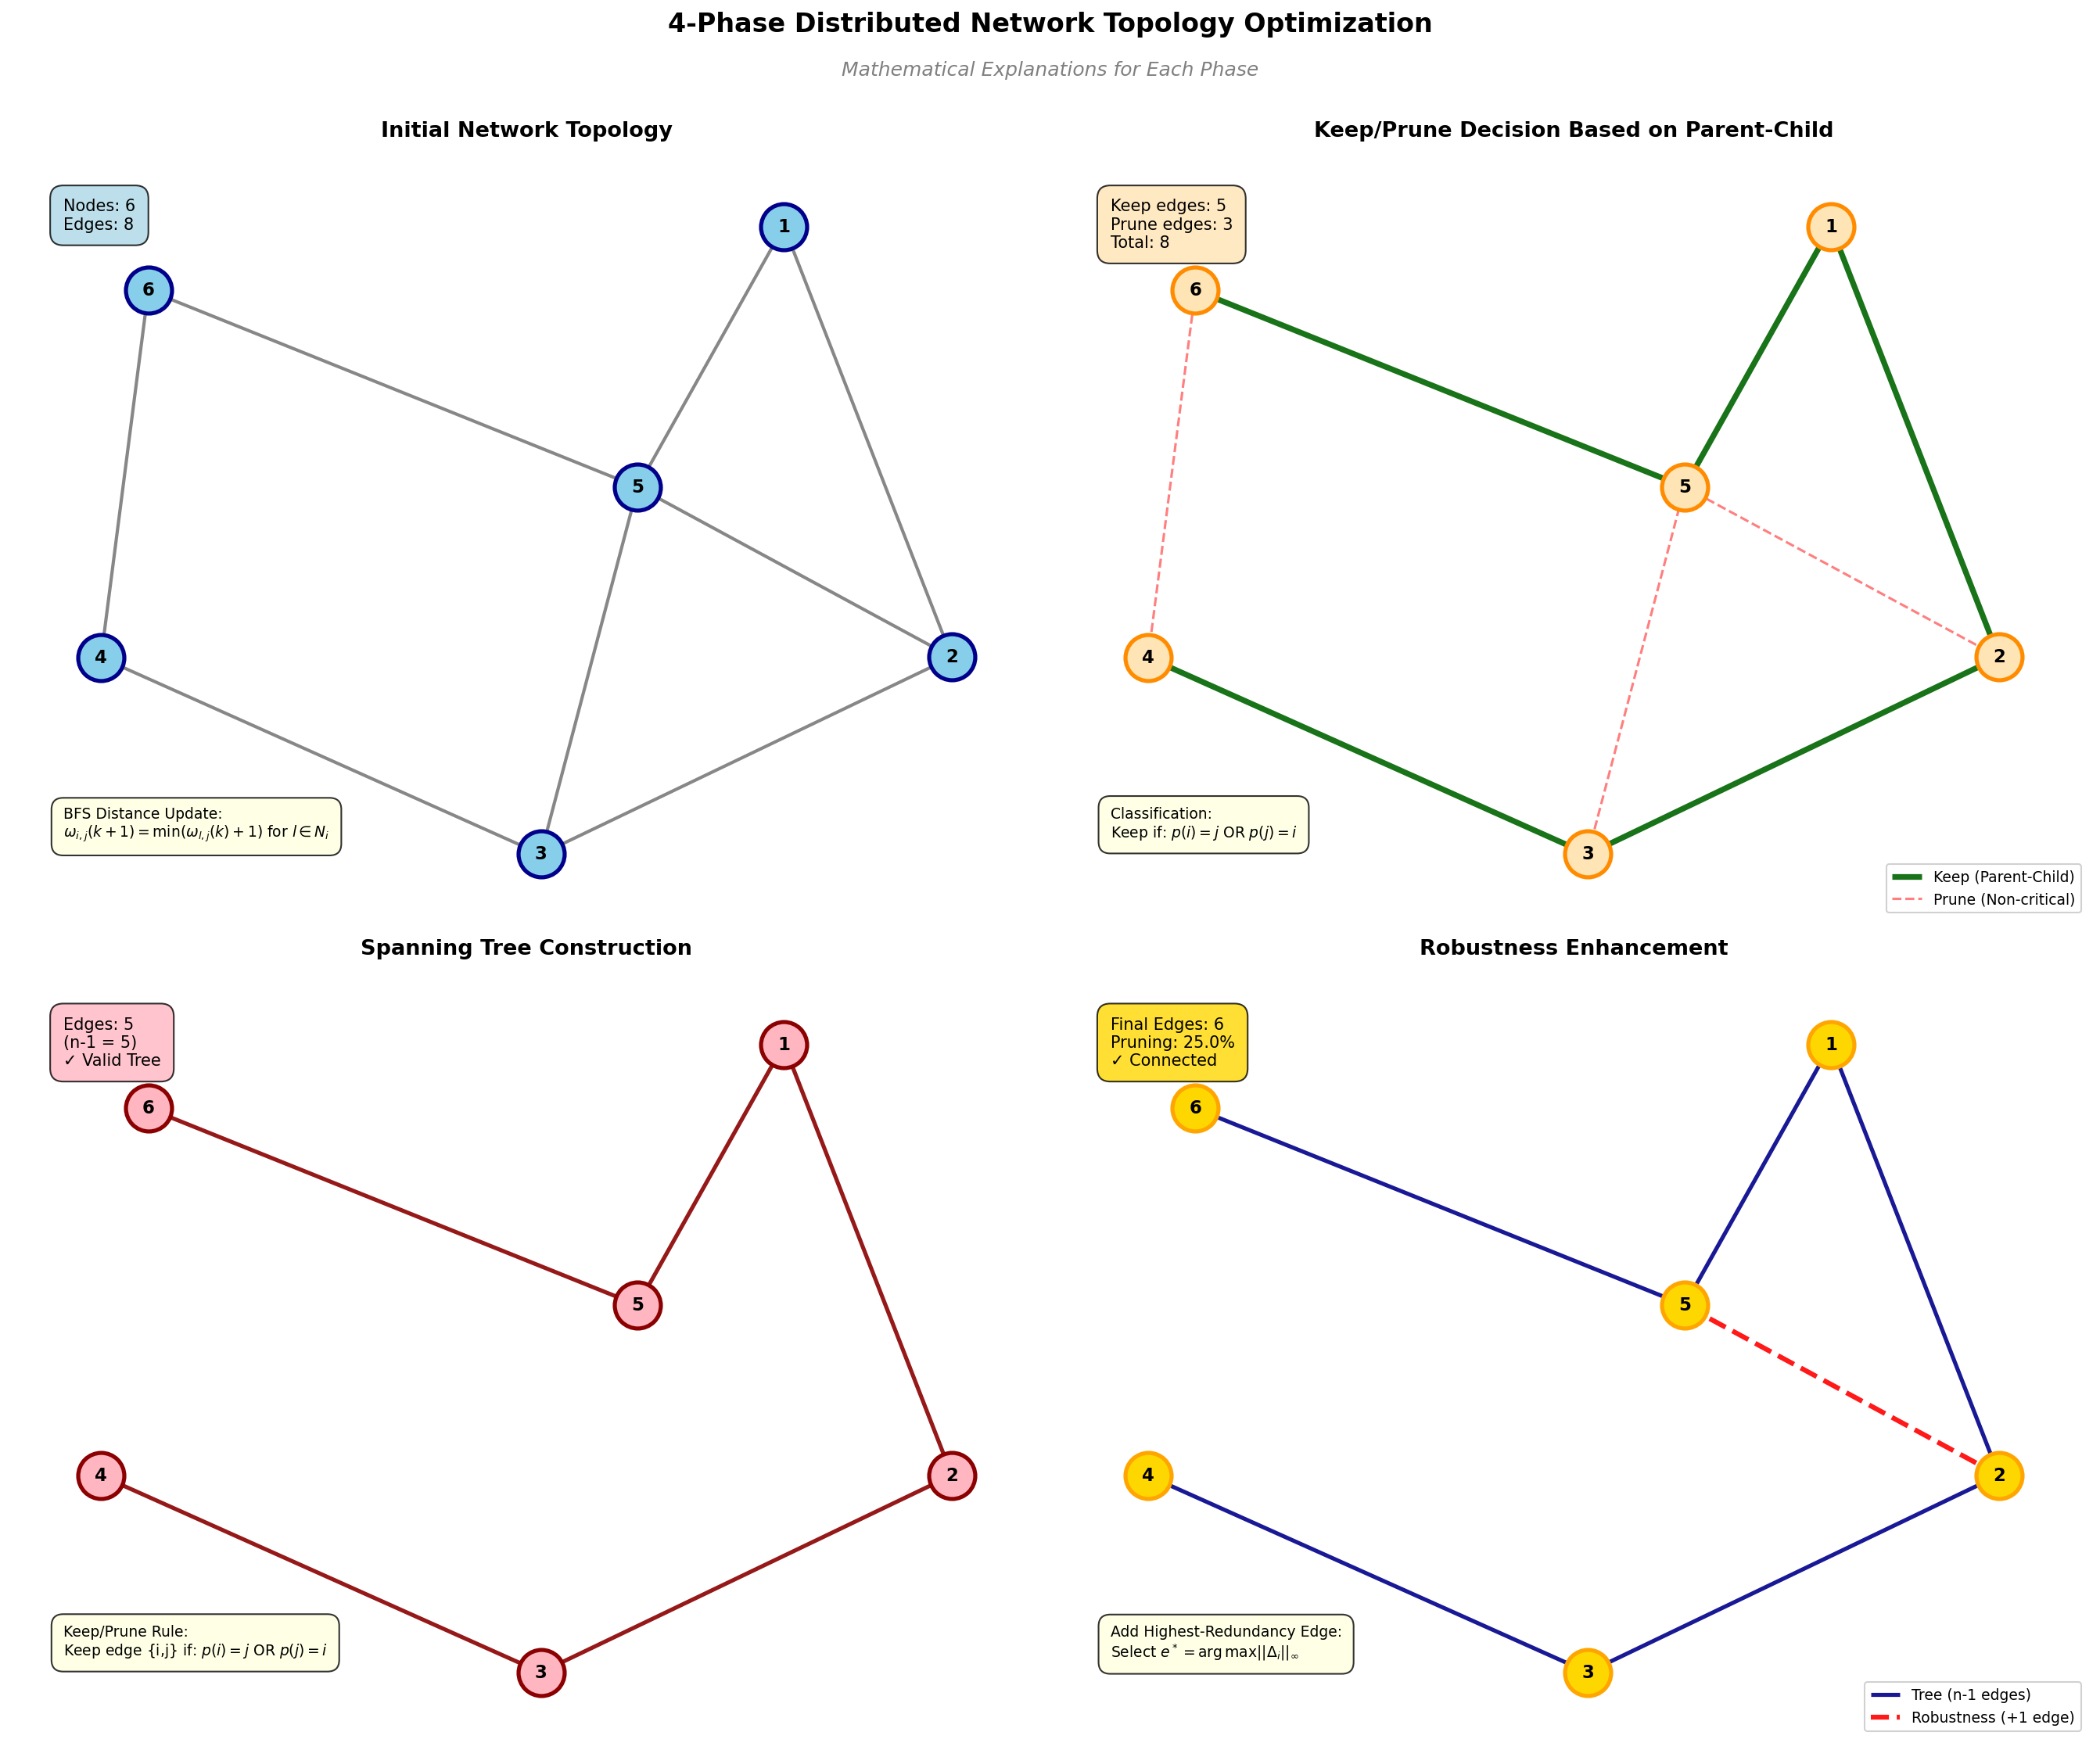
\includegraphics[width=\columnwidth]{figures/phases_2x2_6node_sparse_with_math.png}
\caption{Four-phase evolution on a 6-node sparse network. Phase 1: initial disk-graph topology. Phase 2: Parent Child relation. Phase 3: distributed spanning-tree pruning yields $n-1$ edges. Phase 4 (optional): one additional edge is added to create a single cycle for redundancy.}
\label{fig:example_6node_phases}
\end{figure}

In Fig.\ref{fig:example_6node_phases} we consider $G=(V,E)$ with $V=\{1,2,3,4,5,6\}$, root $r=1$, and
\begin{equation*}
\begin{aligned}
E=\{&(1,2),(2,3),(3,4),(1,5),\\
   &(5,6),(4,6),(2,5),(3,5)\},\\
&|V|=6,\quad |E|=8.
\end{aligned}
\end{equation*}
The neighbor sets are
\begin{equation*}
\begin{aligned}
N_1&=\{2,5\},\quad N_2=\{1,3,5\},\quad N_3=\{2,4,5\},\\
N_4&=\{3,6\},\quad N_5=\{1,2,3,6\},\quad N_6=\{4,5\}.
\end{aligned}
\end{equation*}

Following the distributed hop-distance propagation in~\cite{venkateswaran2024}, robots may compute all-pairs hop distances $\omega_{i,j}$ via local neighbor updates.
In our pruning method we only require distances-to-root, i.e., the scalar $\delta_i=\omega_{i,r}$, which is the $r$-th column of the all-pairs matrix.

Using the converged root distances $\delta_i=\omega_{i,1}$, we obtain
\[
\delta_1=0,\ \delta_2=1,\ \delta_5=1,\ \delta_3=2,\ \delta_6=2,\ \delta_4=3.
\]
Each node selects its parent from neighbors one hop closer to the root:
\[
C_i=\{j\in N_i:\delta_j=\delta_i-1\},\qquad p(i)=\min C_i.
\]
This yields
\[
p(2)=1,\quad p(5)=1,\quad p(3)=2,\quad p(6)=5,\quad p(4)=3,
\]
and the maintained tree edges are the parent edges
\begin{equation*}
\begin{aligned}
E_T=\{&\{1,2\},\{1,5\},\{2,3\},\\
      &\{3,4\},\{5,6\}\},\\
&|E_T|=5=n-1.
\end{aligned}
\end{equation*}
Equivalently, for each $\{i,j\}\in E$ we keep the edge iff $p(i)=j$ or $p(j)=i$.

To introduce a single alternate path, we add one edge based on proximity. Mostly one hope neighbors are considered closest but any application dependent heuristic (e.g., $\{2,5\}$ in Fig.~\ref{fig:example_6node_phases}) can be used to create one redundant cycle.
This step is optional and is not required for the spanning-tree correctness guarantee.

\begin{algorithm}[t]
\caption{Algorithm A: Four-phase distributed pruning with optional redundancy edge}
\label{alg:four_phase_pruning}
\begin{algorithmic}[1]
\REQUIRE Connected disk graph at update time $t_k$ with neighbor sets $N_i(t_k)$; root $r$ (e.g., smallest ID)
\ENSURE Maintained structure $\mathcal{E}_{\mathrm{topo}}(k)$ (tree), optionally plus one redundancy edge

\STATE \textbf{Phase 1 (hop-distance discovery):} run the neighbor propagation~\eqref{eq:omega_update} for $q=0,\dots,n-1$ and set $\delta_i\leftarrow \omega_{i,r}(q^\star)$ as in~\eqref{eq:delta_from_omega}

\STATE \textbf{Phase 2 (monitor):} if $\delta_i=+\infty$ locally, node $i$ declares itself disconnected and triggers a re-run of the update

\STATE \textbf{Phase 3 (core spanning tree):}
\FORALL{nodes $i\neq r$}
    \STATE $C_i \leftarrow \{j\in N_i(t_k): \delta_j=\delta_i-1\}$
    \STATE $p(i)\leftarrow \min C_i$
\ENDFOR
\STATE Keep edge $\{i,j\}$ iff $p(i)=j$ or $p(j)=i$; let $\mathcal{E}_{\mathrm{topo}}(k)\leftarrow \{\{i,j\}\in \mathcal{E}_{t_k}: K_{ij}=1\}$

\STATE \textbf{Phase 4 (optional redundancy):}
\STATE Select one edge $e^\star\in \mathcal{E}_{t_k}\setminus \mathcal{E}_{\mathrm{topo}}(k)$ by a chosen heuristic (e.g., one hop nieighbors)
\STATE $\mathcal{E}_{\mathrm{topo}}(k)\leftarrow \mathcal{E}_{\mathrm{topo}}(k)\cup \{e^\star\}$

\RETURN $\mathcal{E}_{\mathrm{topo}}(k)$
\end{algorithmic}
\end{algorithm}

\subsection{Control layer: CLF goal-seeking with CBF safety \& connectivity maintenance}
Between pruning iterations, each robot runs a CLF--CBF controller under~\eqref{eq:adv-dif}.
The CLF term drives robots toward task goals, while CBF constraints enforce:
(i) \emph{collision avoidance} for all $j\in\mathcal{S}_i(t)$, and
(ii) \emph{range maintenance} for all $j\in\mathcal{T}_i(k)$.

\subsubsection{Barrier functions (pairwise safety and connectivity)}
For any ordered pair $(i,j)$ define $z_{ij}\triangleq x_i-x_j$ and $r_{ij}\triangleq \|z_{ij}\|$.
We use the standard squared-distance barriers
\begin{align}
h^{\mathrm{safe}}_{ij}(x) &\triangleq r_{ij}^2 - d_{\min}^2,
\label{eq:h_safe}\\
h^{\mathrm{conn}}_{ij}(x) &\triangleq R_{\max}^2 - r_{ij}^2,
\label{eq:h_conn}
\end{align}
so that $h^{\mathrm{safe}}_{ij}\ge 0$ implies $\|x_i-x_j\|\ge d_{\min}$ and
$h^{\mathrm{conn}}_{ij}\ge 0$ implies $\|x_i-x_j\|\le R_{\max}$.

To handle spatially varying flow and bounded disturbances (Assumptions in Sec.~\ref{sec:prob}), we employ linear CBF inequalities.
With extended class-$\mathcal{K}$ functions $\alpha_s,\alpha_c$, we enforce robust CBF inequalities using the locally available neighbor-control estimate $\hat u_j$ from Assumption~\ref{ass:A3}.
For each $j\in\mathcal{S}_i(t)$:
\begin{equation}
2 z_{ij}^\top (u_i-\hat u_j)\ \ge\ 2L_f r_{ij}^2 + 4\bar d\, r_{ij}\ -\ \alpha_s\!\big(h^{\mathrm{safe}}_{ij}(x)\big)\ +\ 2 r_{ij}\bar e,
\label{eq:robust_safe_cbf}
\end{equation}
and for each $j\in\mathcal{T}_i(k)$:
\begin{equation}
2 z_{ij}^\top (u_i-\hat u_j)\ \le\ \alpha_c\!\big(h^{\mathrm{conn}}_{ij}(x)\big)\ -\ 2L_f r_{ij}^2 - 4\bar d\, r_{ij}\ -\ 2 r_{ij}\bar e.
\label{eq:robust_conn_cbf}
\end{equation}
The additional $\pm\,2r_{ij}\bar e$ margins ensure correctness under bounded staleness: writing $u_j=\hat u_j+e_{ij}$ with $\|e_{ij}\|\le \bar e$ (Assumption~\ref{ass:A3}), the true relative-control term $2z_{ij}^\top(u_i-u_j)$ differs from $2z_{ij}^\top(u_i-\hat u_j)$ by at most $2r_{ij}\bar e$.

\subsubsection{CLF objective and QP-based safety filter}
Let $x_i^{\mathrm{goal}}(t)$ denote robot $i$'s goal reference.
We adopt the quadratic CLF
\begin{equation}
V_i(x_i) \triangleq \|x_i-x_i^{\mathrm{goal}}(t)\|^2,
\label{eq:clf_V}
\end{equation}
and a nominal goal-seeking command $u_i^{\mathrm{nom}}(t)$.
Robot $i$ then computes a minimally modifying control via a quadratic program:
\begin{align}
u_i^\star(t) = \arg\min_{u_i,\ \sigma_i}\quad &
\|u_i-u_i^{\mathrm{nom}}\|^2 + \rho\,\sigma_i^2
\label{eq:clf_cbf_qp_obj}\\
\text{s.t.}\quad
& \dot V_i(x_i) \le -c V_i(x_i) + \sigma_i
\label{eq:clf_constraint}\\
& \eqref{eq:robust_safe_cbf}\ \ \forall j\in\mathcal{S}_i(t),\qquad
\eqref{eq:robust_conn_cbf}\ \ \forall j\in\mathcal{T}_i(k),
\label{eq:cbf_constraints}\\
& \|u_i\|\le u_{\max}.
\label{eq:input_bound}
\end{align}
The relaxation $\sigma_i$ preserves feasibility when hard constraints dominate; $\rho$ penalizes relaxation.
Crucially, connectivity CBFs are enforced only for the \emph{active} neighbor set $\mathcal{T}_i(k)$, so the number of connectivity constraints scales with the pruned topology rather than the dense disk graph.

\section{Connectivity Preservation Guarantee}
\label{sec:conn_guarantee}

We establish that the maintained coordination subgraph stays connected for all time.
The guarantee is hybrid: (i) continuous-time link feasibility is enforced by staleness-robust connectivity CBF constraints on the maintained edges, and
(ii) discrete-time pruning preserves graph connectivity by constructing a spanning tree from one-hop neighbor messages at each update.

\subsection{Continuous-time maintenance of maintained edges via CBF}
\label{subsec:cbf_link_invariance}

\begin{lemma}
\label{lem:cbf_conn_invariance}
Fix any undirected edge set $\mathcal{E}_c\subseteq \mathcal{V}\times\mathcal{V}$ and define
\[
\mathcal{C}_{\mathrm{conn}}(\mathcal{E}_c)
\triangleq
\Big\{x\in(\mathbb{R}^n)^N:\ \|x_i-x_j\|\le R_{\max},\ \forall (i,j)\in\mathcal{E}_c\Big\}.
\]
Under the dynamics~\eqref{eq:adv-dif} and Assumptions~\ref{ass:A1}--\ref{ass:A4}, suppose that for all $t\ge 0$ and every
$(i,j)\in\mathcal{E}_c$, the applied controls satisfy the staleness-robust connectivity inequality
\begin{equation}
2 z_{ij}^\top (u_i-\hat u_j)\ \le\ \alpha_c\!\big(h^{\mathrm{conn}}_{ij}(x)\big)\ -\ 2L_f r_{ij}^2 - 4\bar d\, r_{ij}\ -\ 2 r_{ij}\bar e,
\label{eq:robust_conn_cbf_recall}
\end{equation}
where $z_{ij}=x_i-x_j$, $r_{ij}=\|z_{ij}\|$, $h^{\mathrm{conn}}_{ij}(x)=R_{\max}^2-r_{ij}^2$, and $\hat u_j$ and $\bar e$ are defined in Assumption~\ref{ass:A3}.
Then $\mathcal{C}_{\mathrm{conn}}(\mathcal{E}_c)$ is forward invariant: if
$x(0)\in\mathcal{C}_{\mathrm{conn}}(\mathcal{E}_c)$, then $x(t)\in\mathcal{C}_{\mathrm{conn}}(\mathcal{E}_c)$ for all $t\ge 0$.
\end{lemma}

\begin{proof}
Let $e_{ij}(t)\triangleq u_j(t)-\hat u_j(t)$, so $\|e_{ij}(t)\|\le \bar e$ by Assumption~\ref{ass:A3}.
Then
\[
2z_{ij}^\top(u_i-u_j)=2z_{ij}^\top(u_i-\hat u_j)-2z_{ij}^\top e_{ij}
\le 2z_{ij}^\top(u_i-\hat u_j)+2r_{ij}\bar e.
\]
Combining with~\eqref{eq:robust_conn_cbf_recall} yields
\[
2z_{ij}^\top(u_i-u_j)\ \le\ \alpha_c\!\big(h^{\mathrm{conn}}_{ij}(x)\big)\ -\ 2L_f r_{ij}^2 - 4\bar d\, r_{ij},
\]
which is the robust connectivity CBF condition for the true applied neighbor control.
Standard CBF arguments then imply forward invariance of $\mathcal{C}_{\mathrm{conn}}(\mathcal{E}_c)$.
\end{proof}

\subsection{Connectivity preservation under pruning updates}
\label{subsec:hybrid_connectivity}

Let $t_k$ denote the $k$-th topology update time. At time $t_k$, the graph layer outputs the maintained edge set $\mathcal{E}_{\mathrm{topo}}(k)$ via the parent-selection and keep rule~\eqref{eq:parent_rule}--\eqref{eq:Etopo_def}.

\begin{theorem}[Connectivity preservation]
\label{thm:hybrid_connectivity}
Assume the initial disk graph $\mathcal{G}_{t_0}=(\mathcal{V},\mathcal{E}_{t_0})$ is connected and Assumption~\ref{ass:A4} holds so that the hop-distance routine~\eqref{eq:omega_update} converges at each update.
At each update time $t_k$, robots prune locally to keep exactly the incident edges in $\mathcal{E}_{\mathrm{topo}}(k)$ defined by~\eqref{eq:Etopo_def}.
Between updates, each robot enforces the staleness-robust connectivity CBF constraints~\eqref{eq:robust_conn_cbf} for all maintained neighbors, i.e., for all $(i,j)\in\mathcal{E}_{\mathrm{topo}}(k)$ on $[t_k,t_{k+1})$.

Then for every $k$:
(i) the maintained graph $(\mathcal{V},\mathcal{E}_{\mathrm{topo}}(k))$ is connected at time $t_k$; and
(ii) all maintained edges satisfy $\|x_i(t)-x_j(t)\|\le R_{\max}$ for all $t\in[t_k,t_{k+1})$.
Consequently, end-to-end connectivity is preserved for all $t\ge t_0$.
\end{theorem}

\begin{proof}
At time $t_k$, Theorem~\ref{thm:tree_pruning_correctness} implies that $(\mathcal{V},\mathcal{E}_{\mathrm{topo}}(k))$ is a spanning tree of $\mathcal{G}_{t_k}$, hence it is connected.

Fix $k$. By Lemma~\ref{lem:cbf_conn_invariance} applied with $\mathcal{E}_c=\mathcal{E}_{\mathrm{topo}}(k)$, enforcing~\eqref{eq:robust_conn_cbf} implies
$\|x_i(t)-x_j(t)\|\le R_{\max}$ for all $(i,j)\in\mathcal{E}_{\mathrm{topo}}(k)$ and all $t\in[t_k,t_{k+1})$.
Therefore each maintained edge remains present in the disk graph throughout $[t_k,t_{k+1})$.
Since the maintained graph is connected at $t_k$ and no maintained edge is lost before $t_{k+1}$, end-to-end connectivity persists on $[t_k,t_{k+1})$.
Repeating for all $k$ establishes the claim for all $t\ge t_0$.
\end{proof}

\section{Simulations and Results}
\label{sec:experiments}

\begin{table}[t]
\centering
\caption{Simulation scenarios and stress factors used in evaluation.}
\label{tab:scenarios}
\setlength{\tabcolsep}{5pt}
\footnotesize
\begin{tabular}{ccccp{0.36\columnwidth}}
\toprule
\textbf{Scenario} & \textbf{$N$} & \textbf{$R_{\max}$ (m)} & \textbf{$\Delta t$ (s)} & \textbf{Purpose} \\
\midrule
A & 10 & 3.0 & 0.05 & Baseline \\
B & 10 & 3.5 & 0.10 & Temporal discretization \\
C & 10 & 2.0 & 0.03 & Sparse-connectivity stress\\
D & 20 & 3.0 & 0.05 & Scalability \\
E & 12 & 2.2 & 0.08 & Extreme stress test\\
\bottomrule
\end{tabular}
\end{table}
\FloatBarrier

\subsection{Simulation setup}
\label{subsec:sim_setup_new}

We evaluate the proposed distributed spanning-tree pruning and CLF--CBF controller in a $10\times 10$\,m$^2$ 2D workspace with a spatially varying flow field.
Robots evolve under the discrete-time approximation of~\eqref{eq:adv-dif},
\begin{equation}
x_i[k{+}1]
=
x_i[k]
+
\Delta t\Big(f_{\mathrm{flow}}(x_i[k],k\Delta t) + u_i[k] + d_i[k]\Big),
\label{eq:sim_euler}
\end{equation}
with bounded input $\|u_i\|\le u_{\max}$ and bounded disturbance $\|d_i\|\le \bar d$.
The communication graph is the disk graph~\eqref{eq:disk_graph}--\eqref{eq:neighbors} with range $R_{\max}$.
We run five scenarios and compare four maintained-topology strategies:
\begin{itemize}
  \item \textbf{Fully Connected}: no pruning, $\mathcal{E}_{\mathrm{topo}}(k)=\mathcal{E}_{t_k}$.
  \item \textbf{Centralized MST}: an offline centralized MST (used only as a comparison oracle).
  \item \textbf{Adjacency Consensus}: a sequential pruning baseline (edge removals applied iteratively).
  \item \textbf{Distributed Pruning (ours)}: the distributed hop-distance routine~\eqref{eq:omega_update} followed by spanning-tree pruning~\eqref{eq:parent_rule}--\eqref{eq:Etopo_def}.
\end{itemize}

\paragraph{Topology-update execution}
At each topology update time $t_k$, robots run~\eqref{eq:omega_update} for $q=0,\dots,n-1$ rounds using one-hop message exchange, compute $\delta_i=\omega_{i,r}$, select parent pointers via~\eqref{eq:parent_rule}, and prune locally using~\eqref{eq:keep_indicator}--\eqref{eq:Etopo_def}.
This produces a maintained spanning tree with $|\mathcal{E}_{\mathrm{topo}}(k)|=N-1$ edges.
Between topology updates, robots enforce connectivity CBF constraints only on maintained neighbors $\mathcal{T}_i(k)$ and collision-avoidance constraints on $\mathcal{S}_i(t)$.

\paragraph{Evaluation protocol}
We run a total of 40 simulations of 5 scenarios $\times$ 4 methods $\times$ 2 Monte-Carlo trials, each for 10\,s with sampling at 0.1\,s (100 evaluation points).

\subsection{Metrics}
A run is considered successful if the maintained graph remains connected for the full duration (verified by a connectivity check on $\mathcal{G}_{\mathrm{topo}}(t)$).
We report:
\begin{itemize}
  \item \textbf{Edge reduction (\%)}: $((E_0-E_f)/E_0)\times 100\%$. 
  \item \textbf{Edge-count trajectory} $E(t)$ over time.
  \item \textbf{Offline diagnostic connectivity margin}: minimum algebraic connectivity.
\end{itemize}

Table~\ref{tab:scenarios} summarizes five test scenarios with varying parameters to validate robustness: 
Scenario A, B (large time step $\Delta t{=}0.2$\,s), C (tight communication radius $R_{\mathrm{comm}}{=}2.0$\,m), 
D (high robot count $n{=}20$), and E (combined extreme parameters).

\begin{figure}[t]
\centering
\begin{minipage}[b]{0.48\columnwidth}
\centering
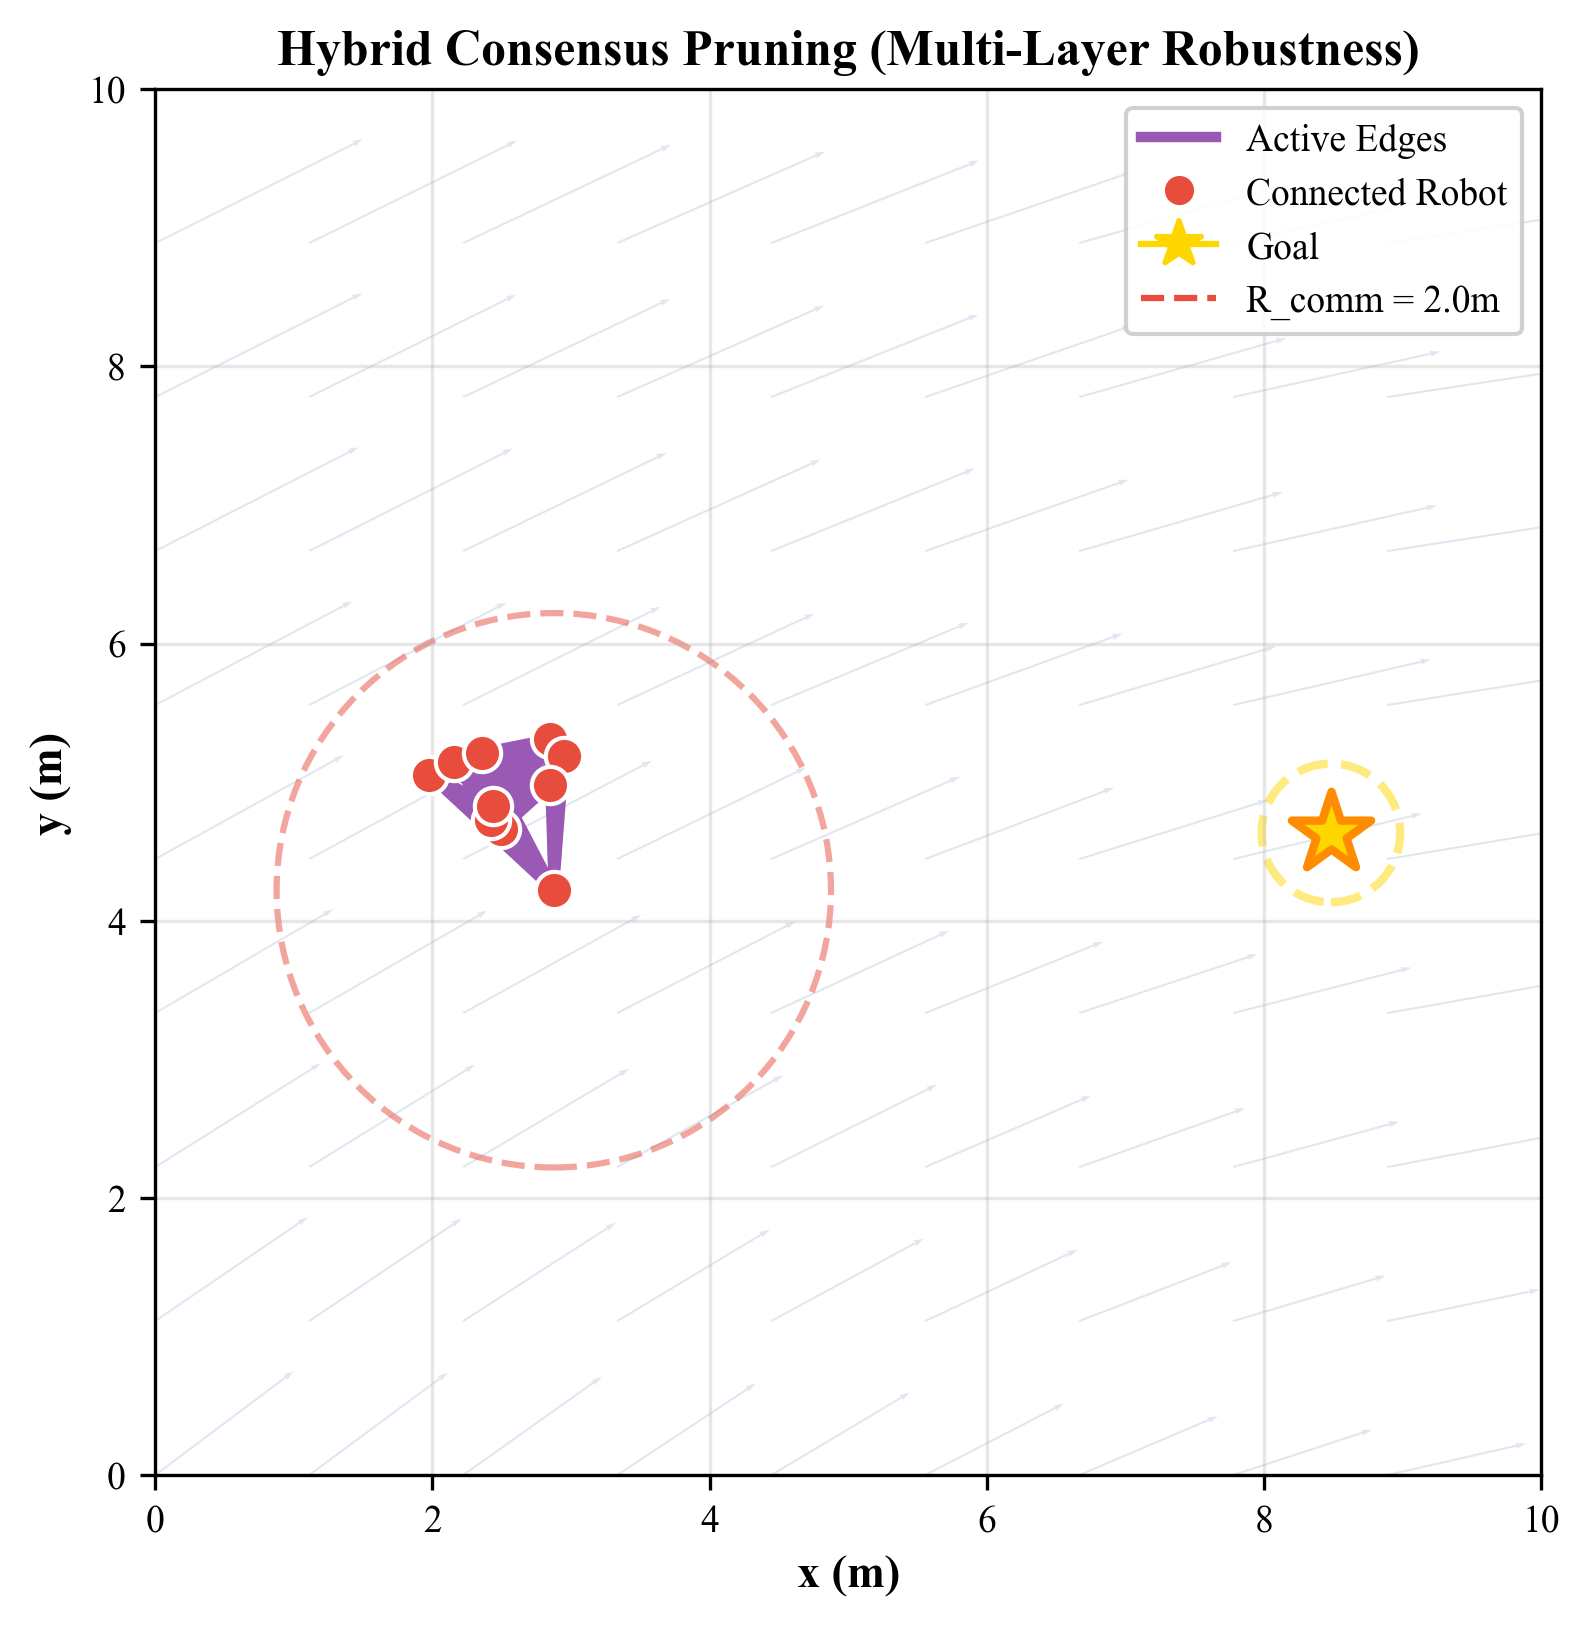
\includegraphics[width=\textwidth]{figures/figure1_acc2026.png}
\caption{Illustrative snapshot showing maintained topology: the fleet advances toward the goal while the pruning layer maintains a sparse, connectivity-feasible subgraph.}
\label{fig:overview_pruning}
\end{minipage}
\hfill
\begin{minipage}[b]{0.48\columnwidth}
\centering
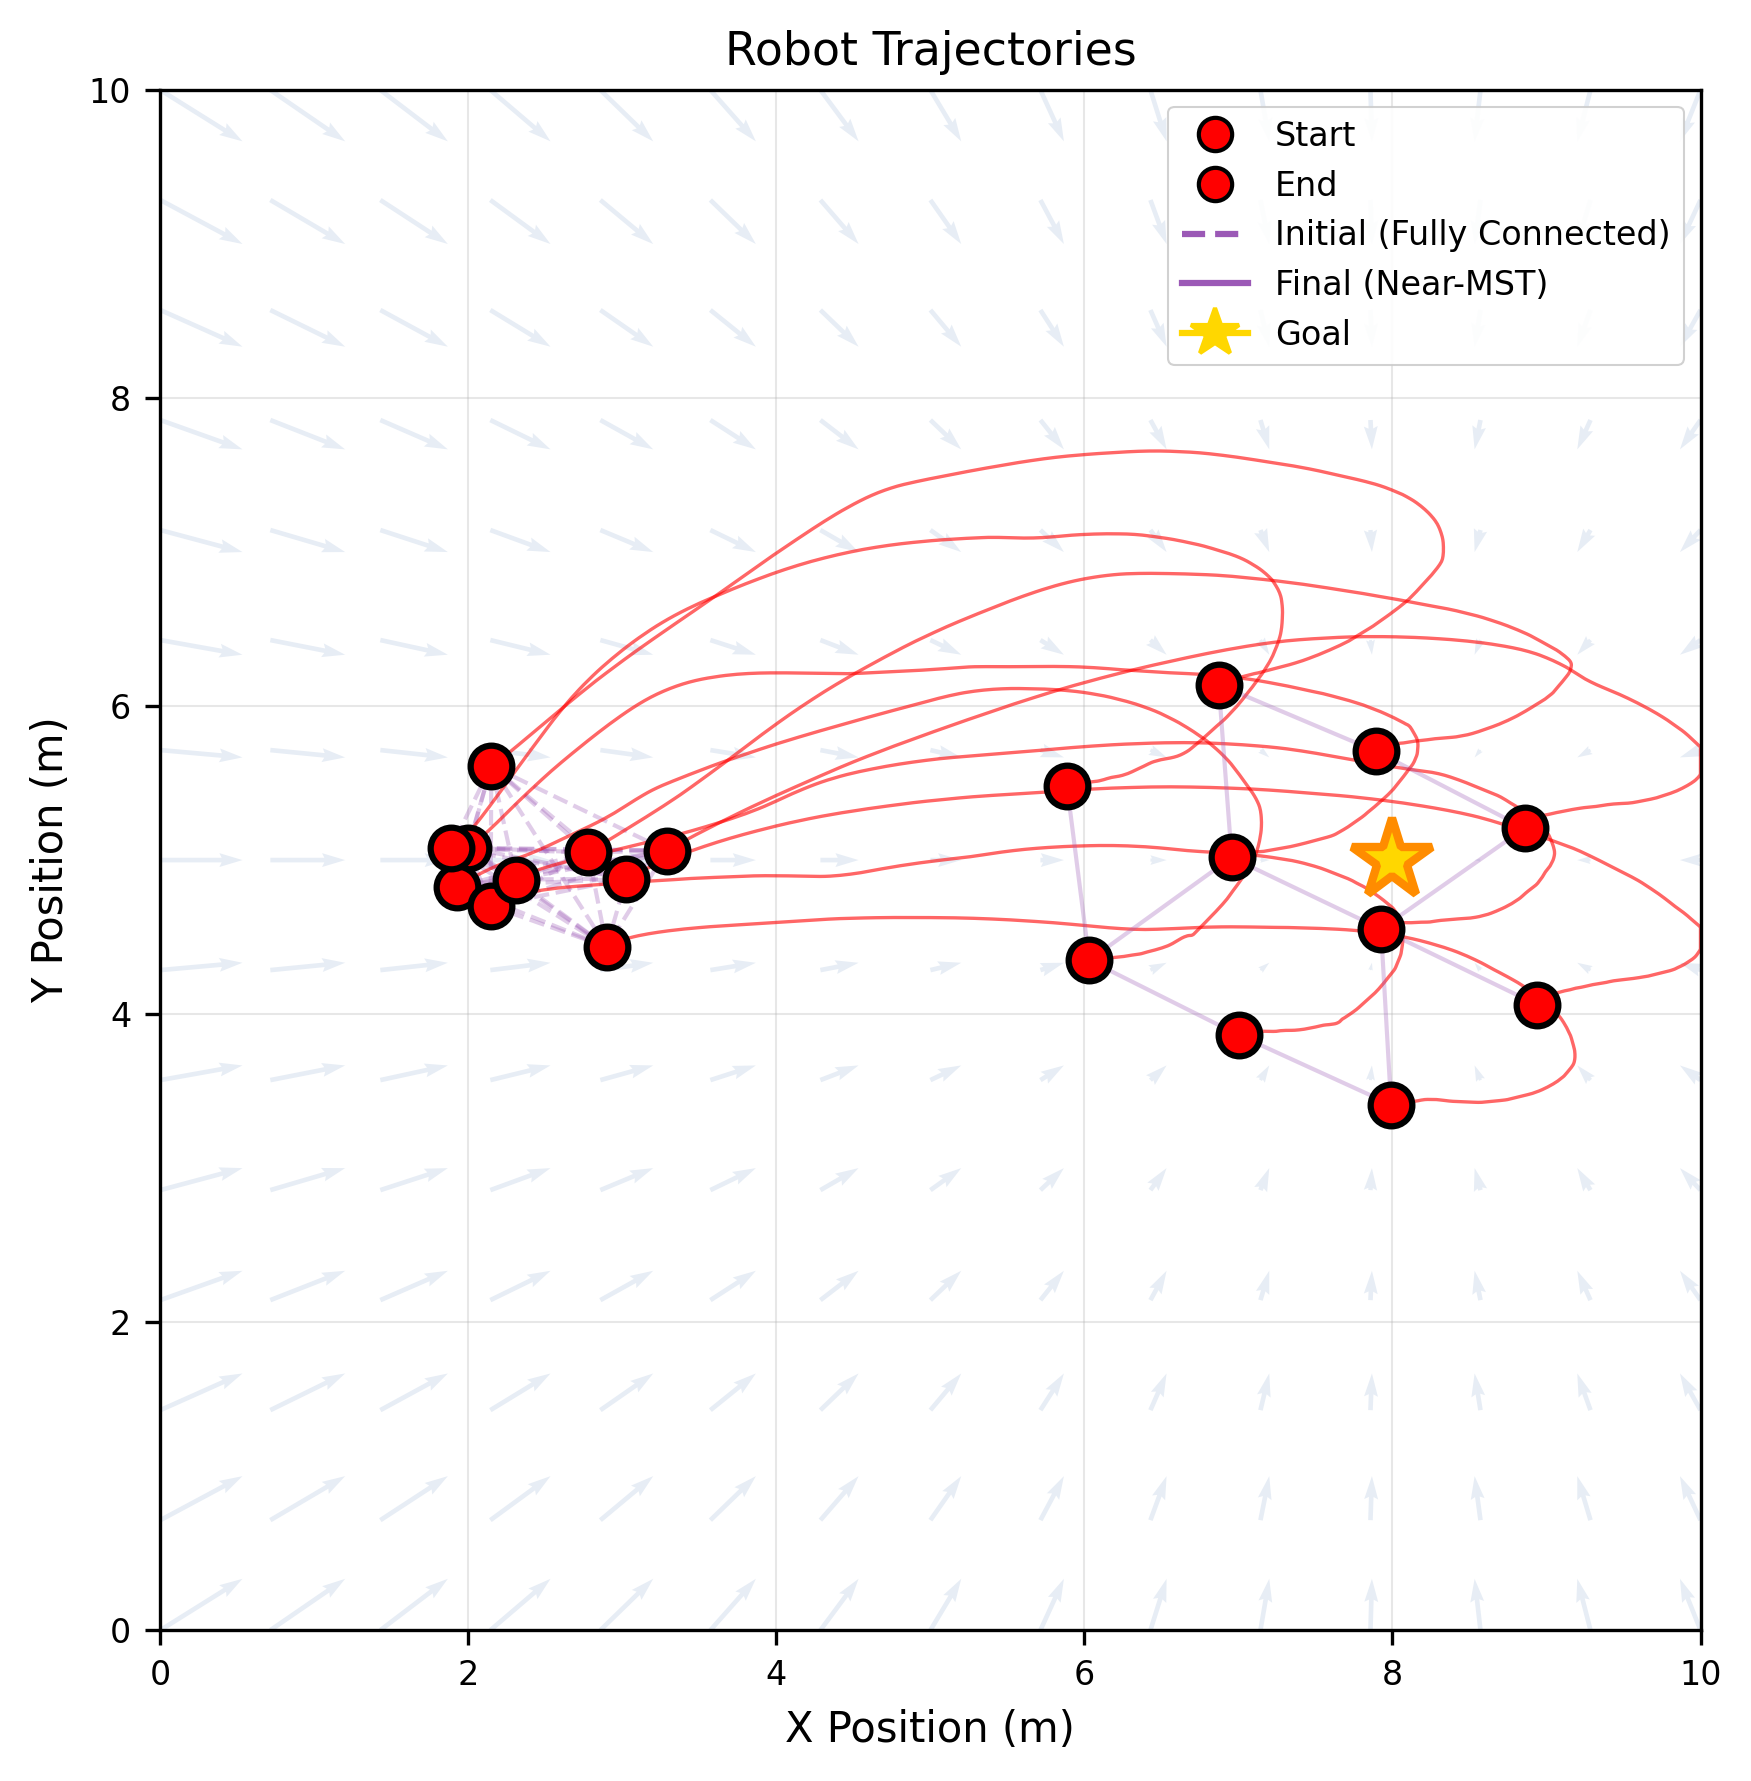
\includegraphics[width=\textwidth]{figures/plot_1_trajectories.png}
\caption{Robot trajectories (Scenario A) in the flow field with topology evolving from initially dense (dashed) to sparse near-tree (solid).}
\label{fig:traj_scnA}
\end{minipage}
\end{figure}

\section{Results}
\label{sec:results}

\paragraph{Qualitative behavior.}
Fig.~\ref{fig:overview_pruning} and Fig.~\ref{fig:traj_scnA} shows representative trajectories in the flow field for Scenario A.
The proposed method maintains only a sparse spanning-tree structure while the team disperses and moves toward the goal.

\paragraph{Edge reduction across scenarios.}
Fig.~\ref{fig:edge_reduction_across} and Fig.~\ref{fig:dp_all_scen} compares final edge reduction across scenarios.
Across all runs, DistributedPruning achieves strong edge reduction while preserving connectivity: on average 72.0\% edge reduction (mean across trials), close to the centralized MST (80.2\%) and higher than the AdjacencyConsensus baseline (67.5\%).

\begin{figure}[t]
\centering
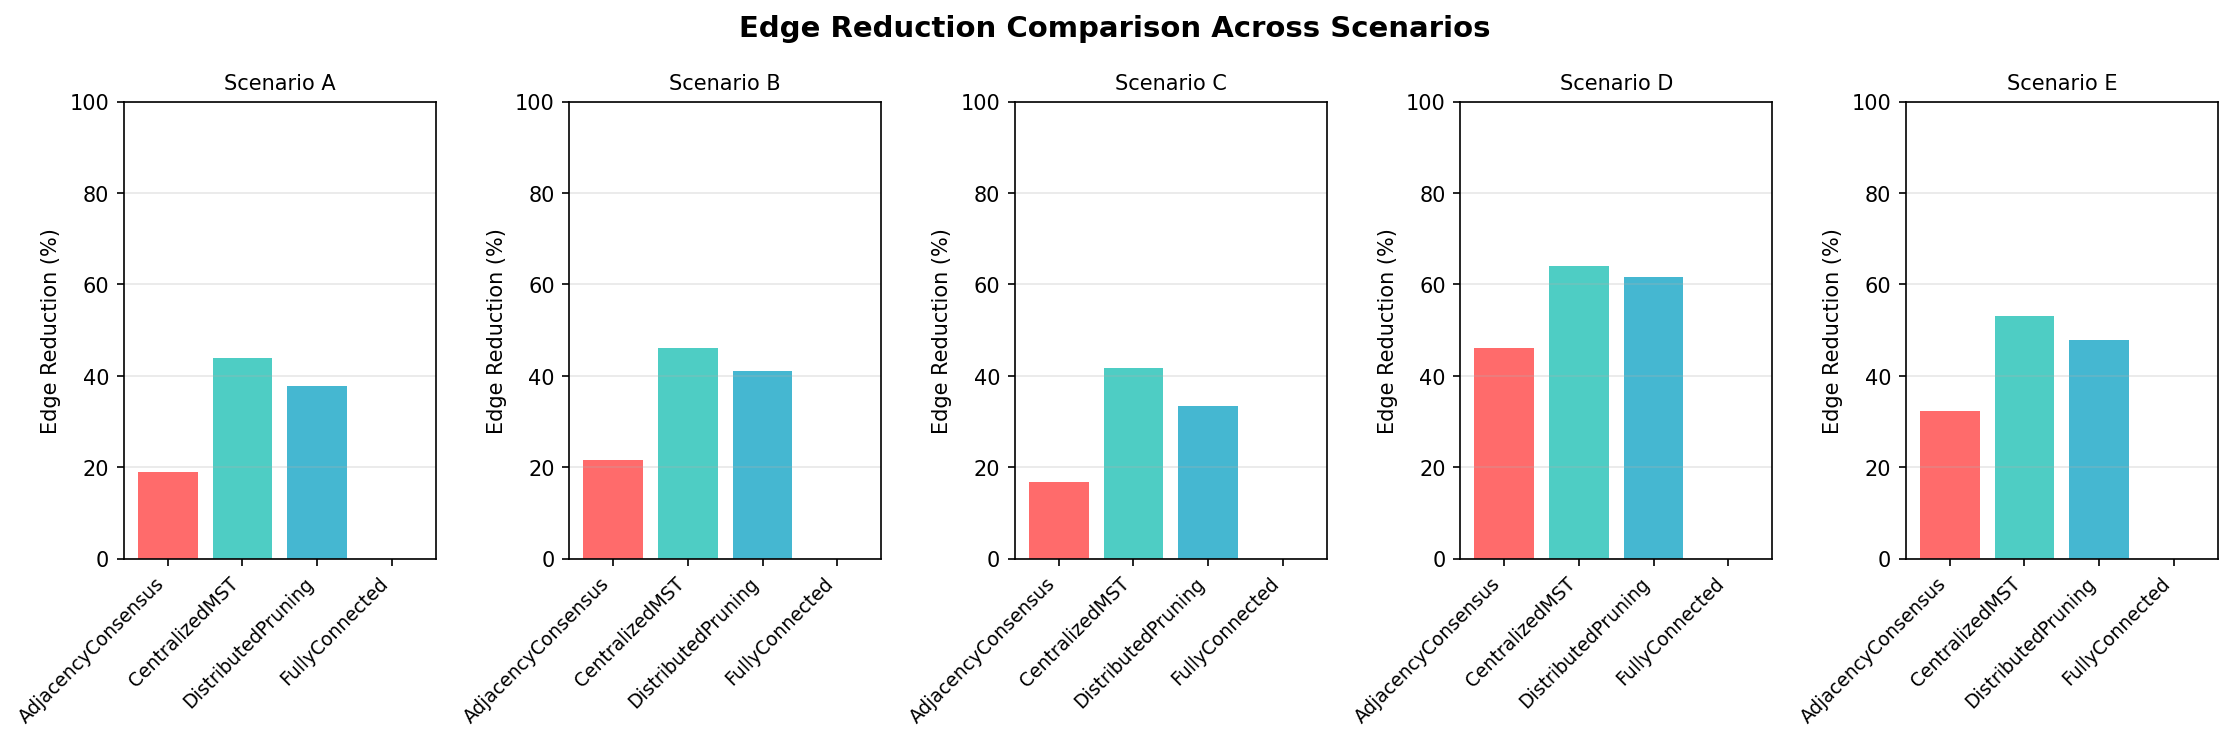
\includegraphics[width=\columnwidth]{figures/01_edge_reduction.png}
\caption{Edge reduction comparison across scenarios for four topology strategies.}
\label{fig:edge_reduction_across}
\end{figure}

\paragraph{Edge-count evolution over time.}
Fig.~\ref{fig:edge_timeseries} shows edge-count evolution in Scenario A, while Fig.~\ref{fig:dp_all_scen} summarizes the edge-count time series for DistributedPruning across all five scenarios.
DistributedPruning transitions from the initially dense topology to a near-tree structure quickly and remains sparse thereafter.

\begin{figure}[t]
\centering
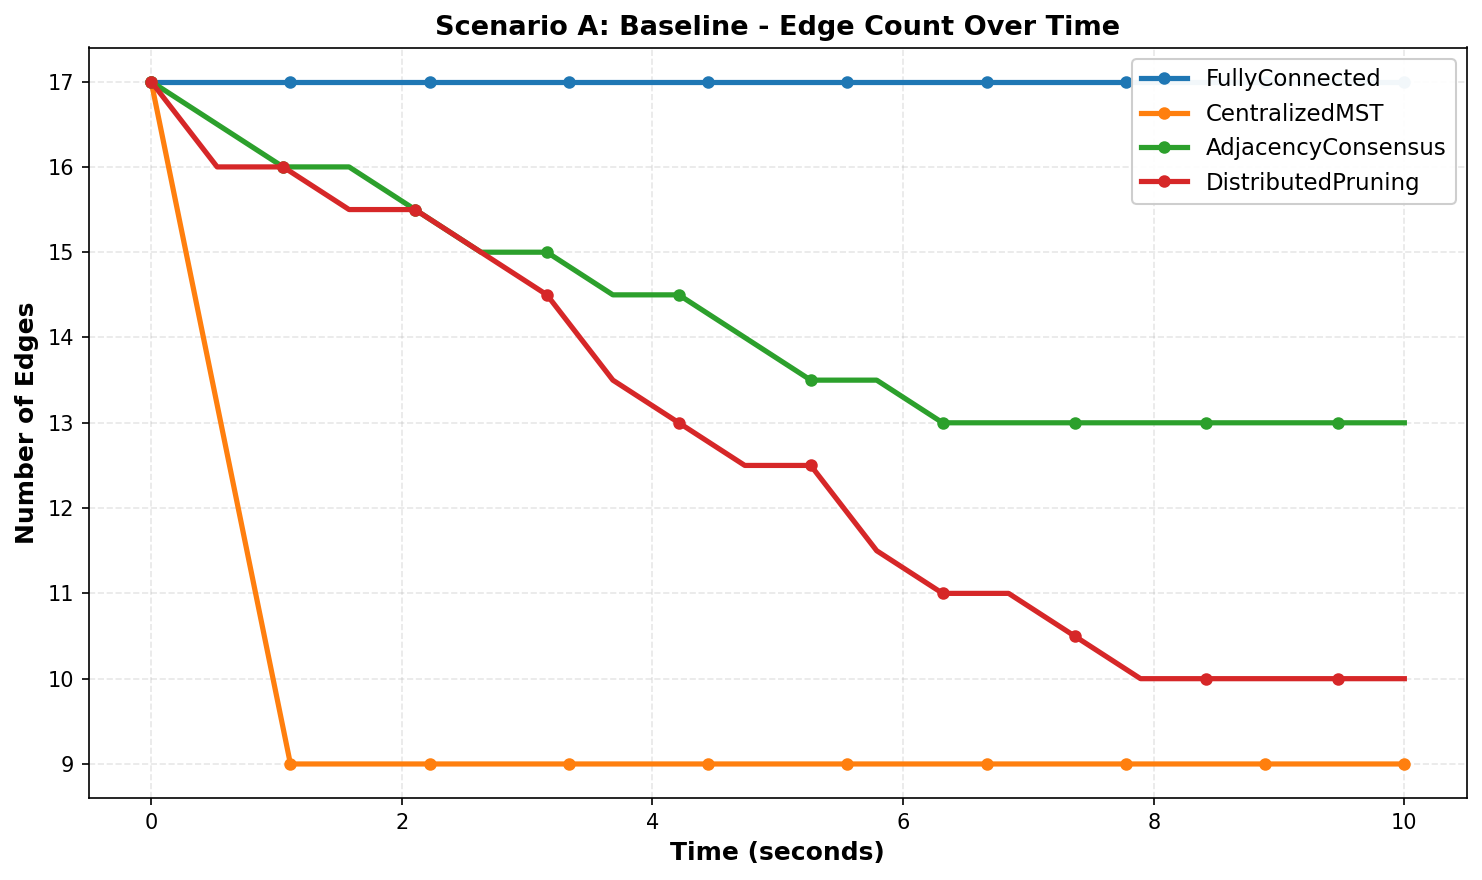
\includegraphics[width=\columnwidth]{figures/simple_timeseries.png}
\caption{Scenario A: maintained edge count $E(t)$ over time for four topology strategies.}
\label{fig:edge_timeseries}
\end{figure}

\begin{figure}[t]
\centering
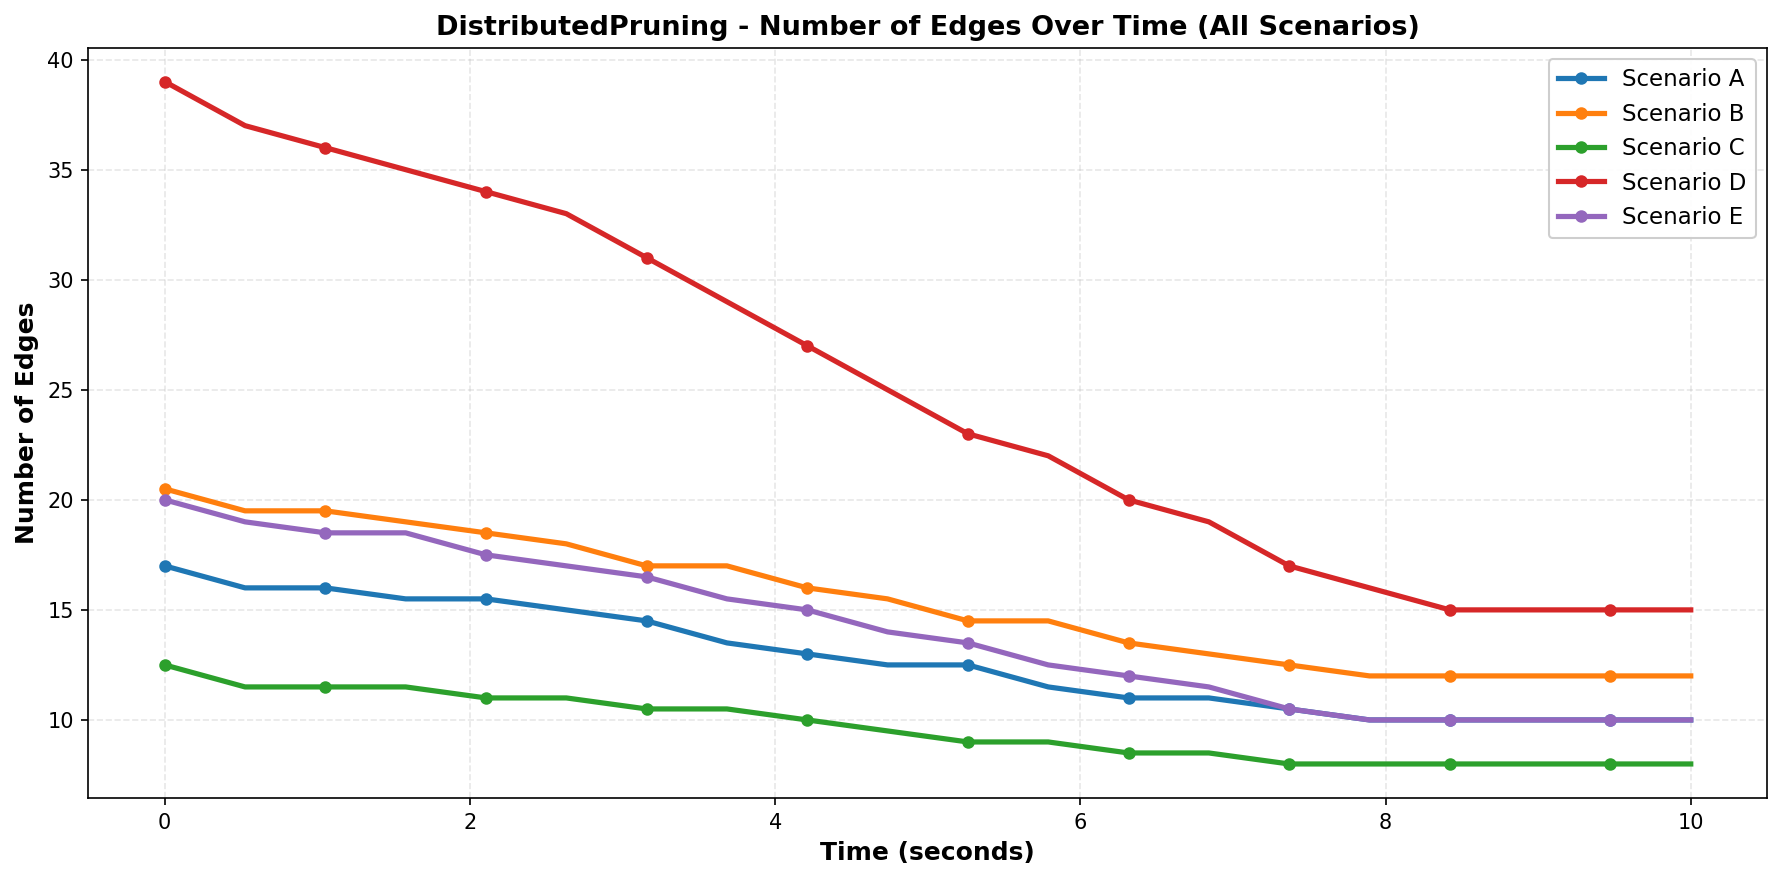
\includegraphics[width=\columnwidth]{figures/distributed_pruning_line_plot.png}
\caption{DistributedPruning: maintained edge count $E(t)$ over time across scenarios.}
\label{fig:dp_all_scen}
\end{figure}

\paragraph{Aggregate statistics (all scenarios).}
Across all 40 experiments, DistributedPruning achieves 97.5\% success, with 72.04\%$\pm$14.2\% edge reduction (mean$\pm$std).
The centralized MST is slightly less reliable (92.0\%) but provides a strong sparsity comparison point.
We additionally report $\min_t\lambda_2$ as an offline diagnostic connectivity margin.

\begin{table}[H]
\centering
\caption{Aggregate performance across all scenarios}
\label{tab:summary_stats}
\footnotesize
\setlength{\tabcolsep}{2.4pt}
\resizebox{\columnwidth}{!}{%
\begin{tabular}{lcccc}
\toprule
Method & Success (\%) & Edge red.\ (\%) & $\min_t \lambda_2$ & Runtime (s) \\
\midrule
Distributed Pruning (Our) & 97.83 & $72.04\pm 14.17$ & $0.7276\pm 1.1044$ & $3.73\pm 4.95$ \\
Adjacency Consensus & 98.21 & $67.20\pm 15.47$ & $0.8297\pm 0.9205$ & $12.91\pm 17.68$ \\
Full Graph & 98.78 & $25.48\pm 20.18$ & $2.0786\pm 1.1935$ & $1.33\pm 0.77$ \\
Centralized MST & 92.02 & $80.57\pm 4.24$ & $0.1500\pm 0.0727$ & $1.00\pm 0.62$ \\
\bottomrule
\end{tabular}}
\end{table}
\FloatBarrier

\section{Conclusion}
\label{sec:conclusion}

We presented a fully distributed framework for connectivity-preserving deployment of flow-driven robot fleets under limited communication.
At discrete update times, robots exchange only neighbor messages to compute hop-distance estimates and prune the dense disk graph to a maintained spanning-tree coordination structure.
A distributed CLF--CBF safety filter enforces collision avoidance and maintains the range constraints of the maintained links under bounded disturbances and bounded neighbor-control staleness.
The resulting hybrid system preserves end-to-end connectivity while substantially reducing the number of maintained edges and associated communication constraints.

Simulations across multiple network scenarios demonstrate that the proposed distributed pruning achieves strong edge reduction while maintaining high success rates, and performs competitively relative to centralized and sequential method baselines.
Future work will (i) incorporate explicit packet-drop models and fully asynchronous update protocols, (ii) extend evaluation to 3D flows, and (iii) validate the framework on field robotic platforms operating in real currents.

\bibliographystyle{IEEEtran}
\bibliography{bibliography}

\end{document}
